\textbf{Solution:}

\begin{figure}[h!]
    \centering
    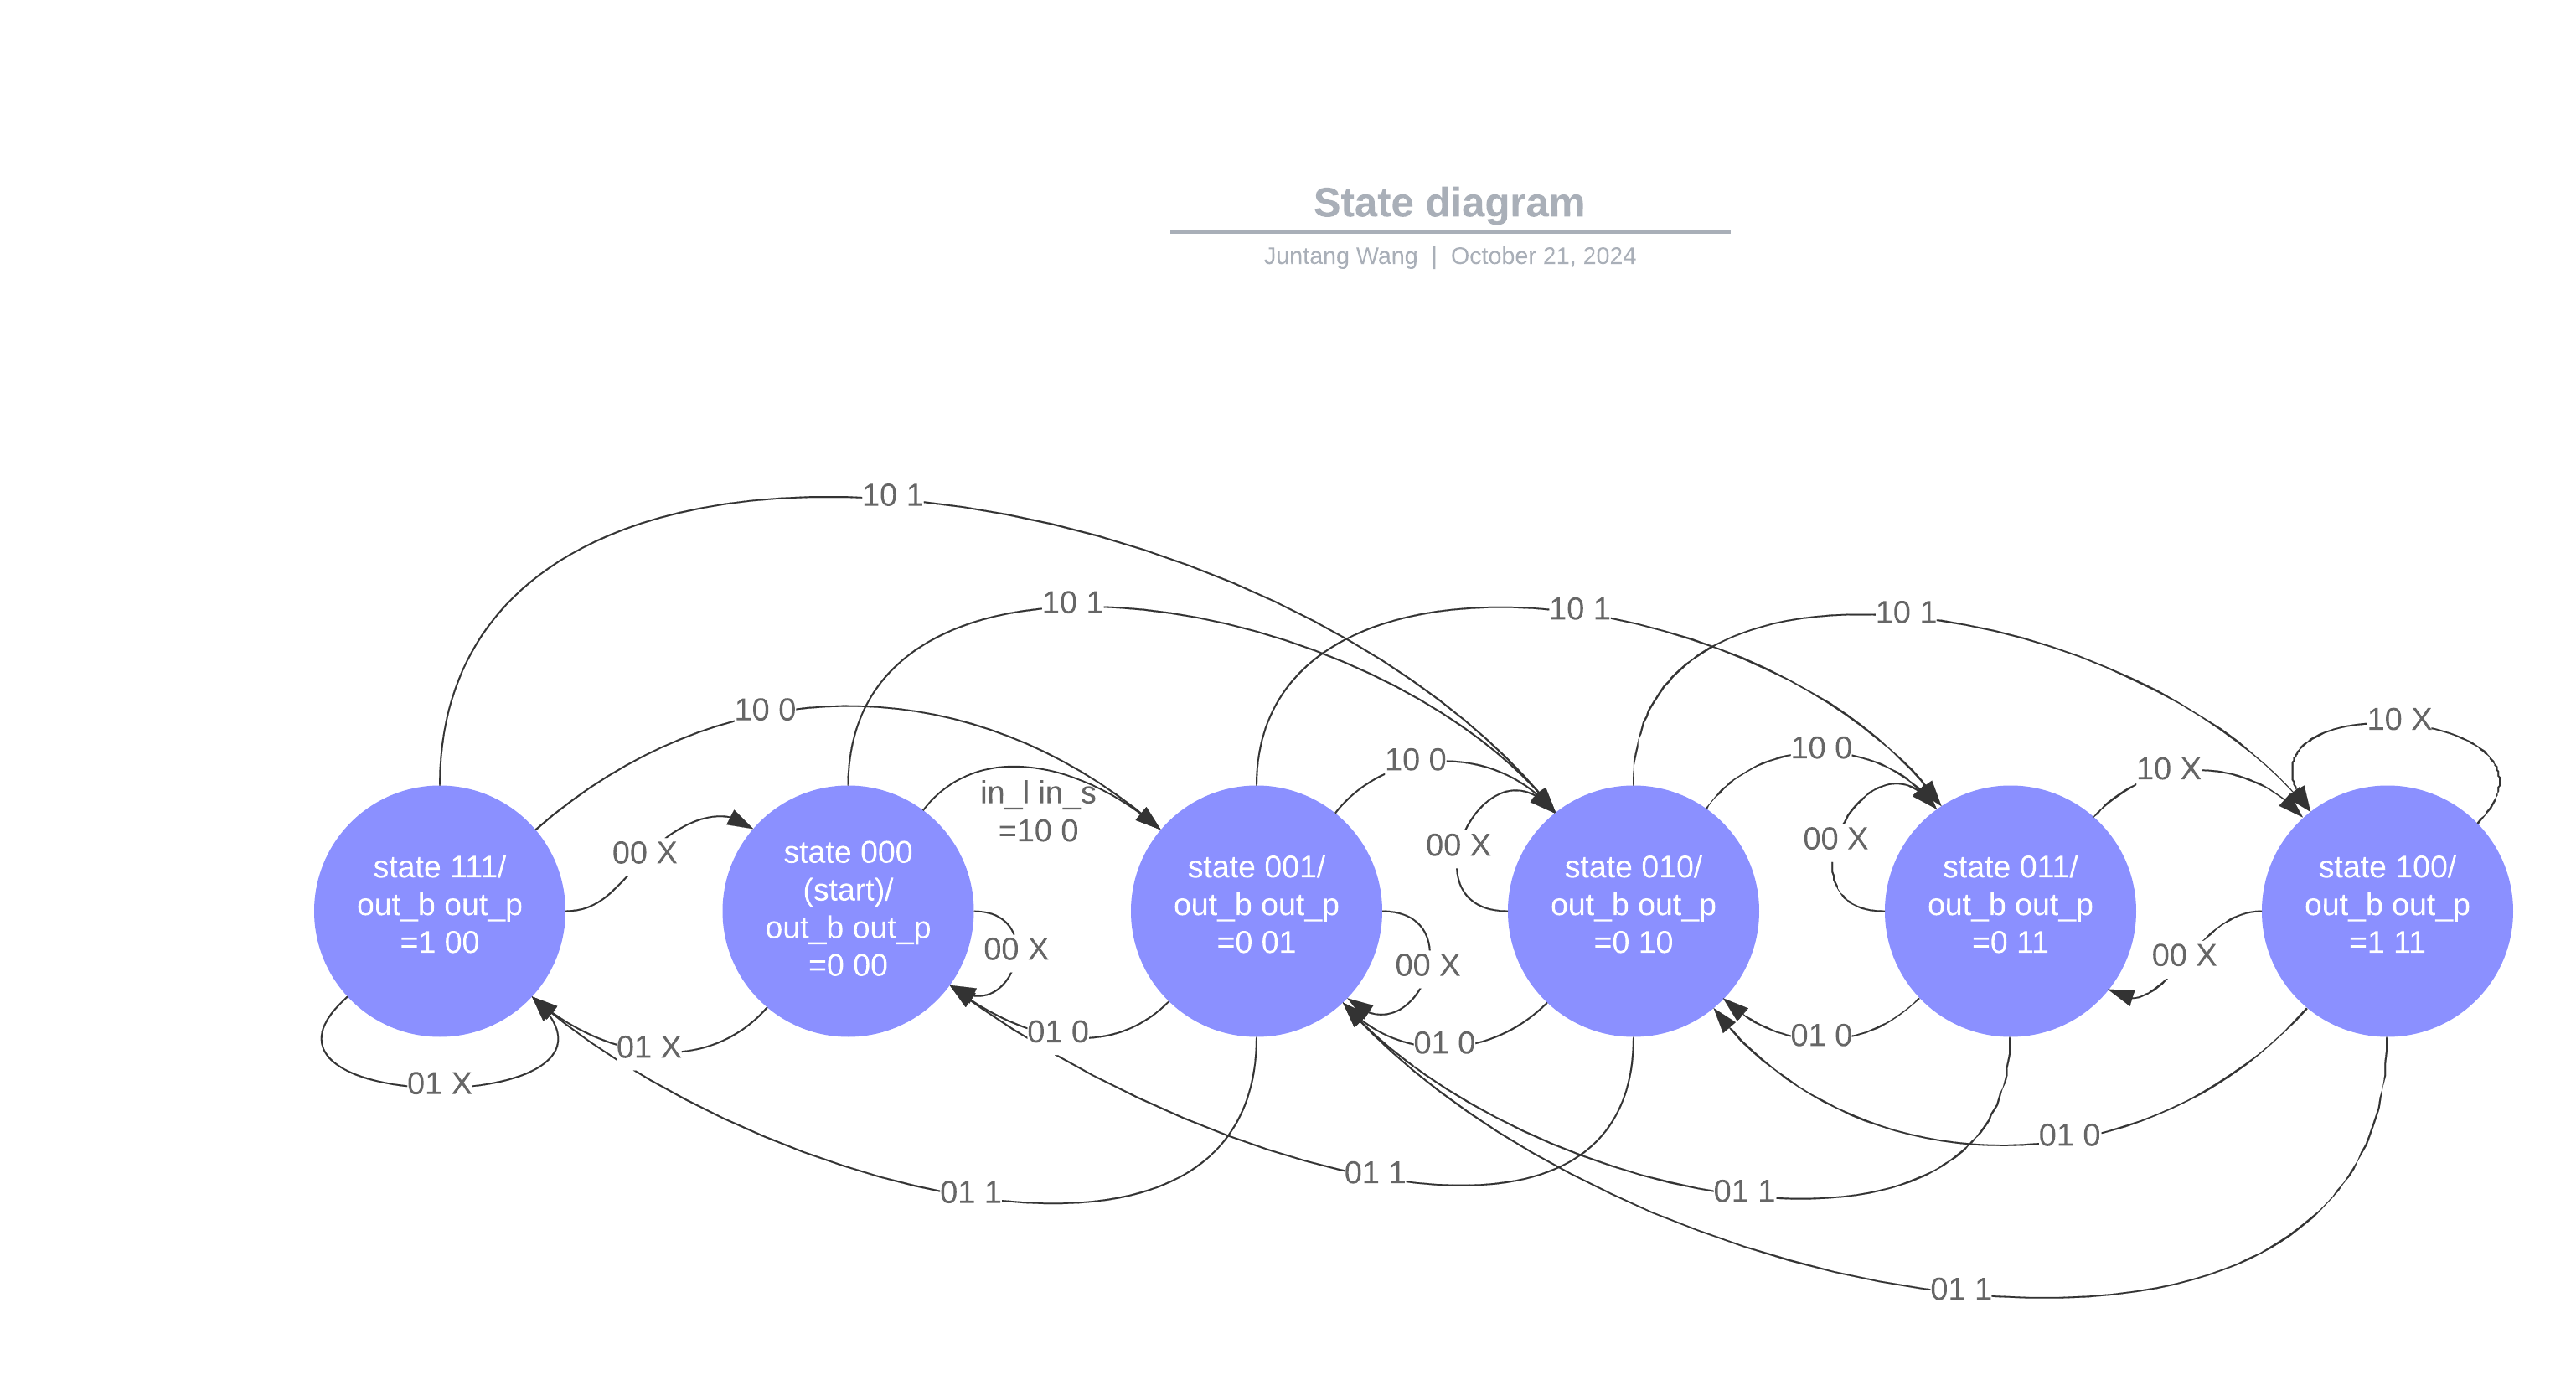
\includegraphics[width=0.8\textwidth]{figures/State diagram.png}
    \caption{State diagram for the FSM}
    \label{fig:state-diagram}
\end{figure}

Figure \ref{fig:state-diagram} shows the state diagram for the finite state machine (FSM). This diagram illustrates the states and transitions of the FSM based on the given specifications.

\begin{itemize}
    \item The FSM has six states: 100, 000, 001, 010, 011 and 111.
    \item Transitions between states occur based on the input\_leftright (input\_l) and input\_speed (input\_s).
    \item The output\_position (output\_p) and output\_blocked (output\_b) is determined by the current state.
\end{itemize}

The state diagram was created using Lucid Chart \cite{lucidchart}.

% ----------------------------------------------------------------
% Drafted by Juntang Wang 2024-10-21
% ----------------------------------------------------------------  
